\documentclass[10pt,pscyr,nonums]{hedlab}
\usepackage[russian]{babel}
\usepackage{hedmaths}
\usepackage{graphicx}
\graphicspath{{plots/}, {images/}}

\newgeometry{top=1.5cm, bottom=1.5cm, left=1cm, right=1cm}

\student{} \date{}
\labnum{5}
\labname{Определение параметров тиратрона}
\begin{document}
    \makeheader

    \emph{Цель работы:} знакомство с управляемыми газоразрядными приборами,
    построение вольтамперной и пусковой характеристик тиратрона.
    
    \begin{figure}[h!]
        \center
        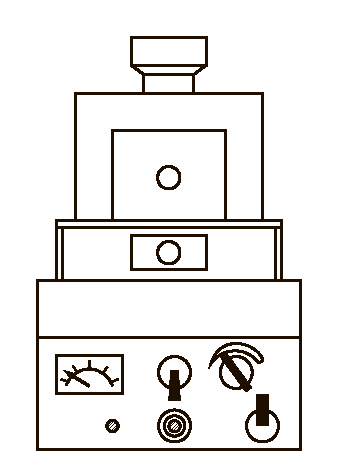
\includegraphics[width=.37\textwidth]{appearance} \hspace*{2em}
        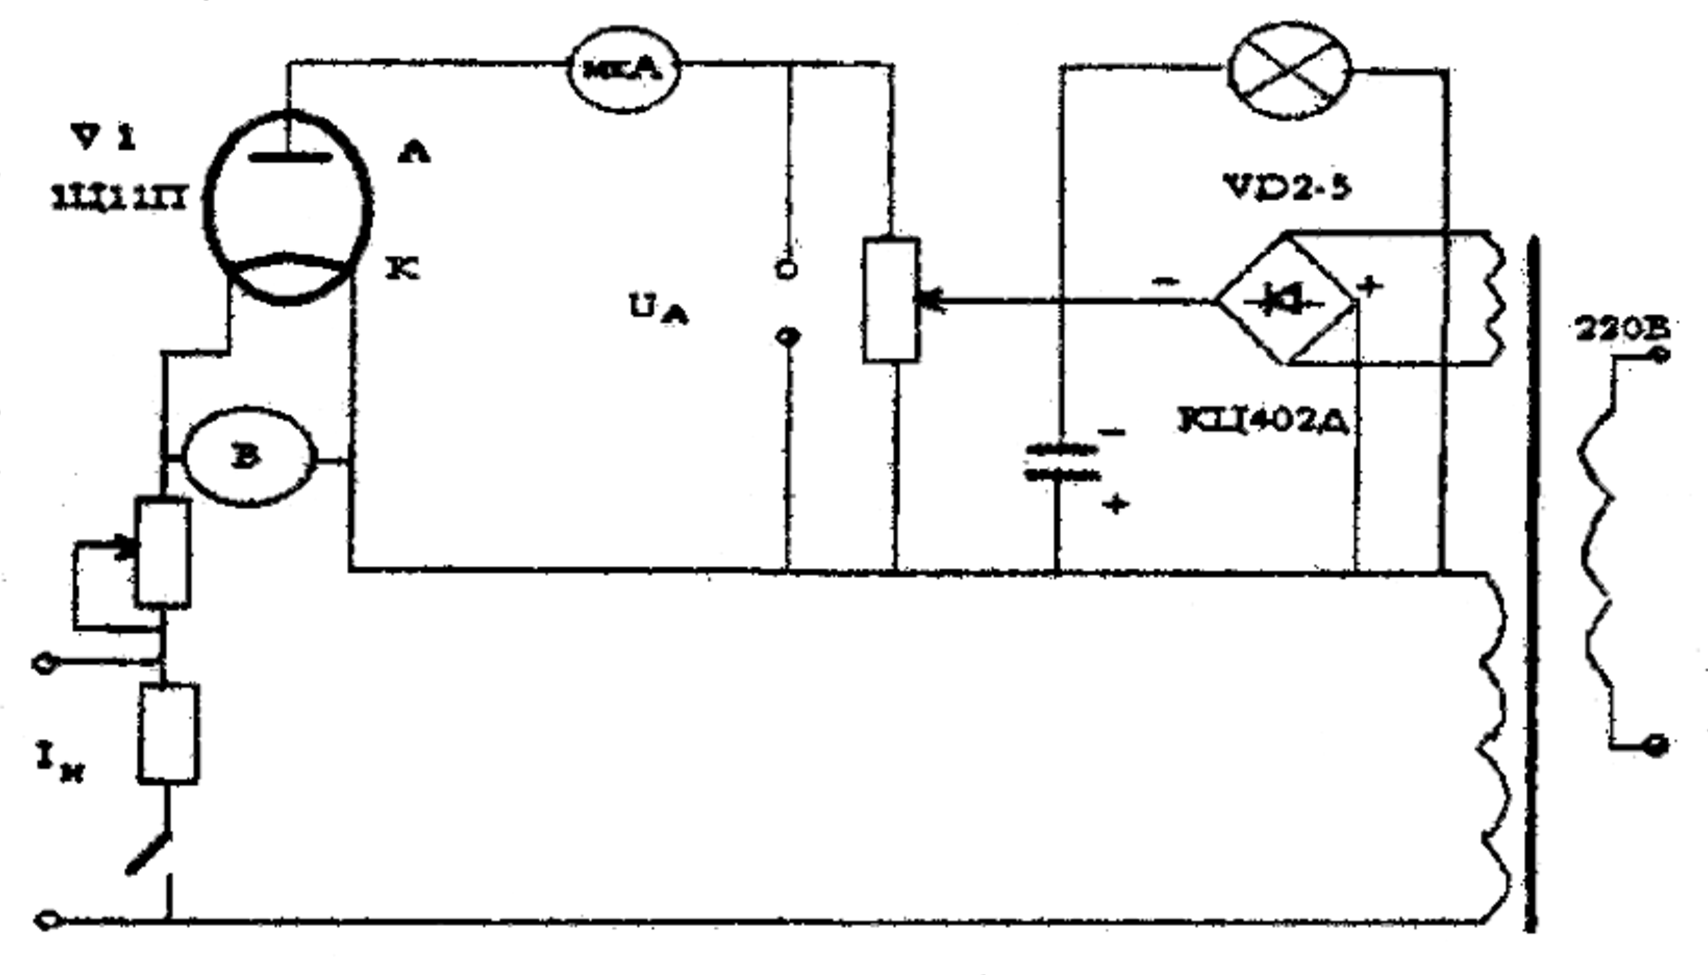
\includegraphics[width=.45\textwidth]{scheme}
        \parbox{.37\textwidth}{\caption{Лабораторная установка}}
        \hspace*{2em}
        \parbox{.45\textwidth}{\caption{Принципиальная схема установки}}
    \end{figure}
    
    \begin{table}[h!]
        \center
        \caption{Пусковая характеристика тиратрона}
        \begin{tabular}{|r|*{6}{C{.07}|}} \hline
            \( U_c \), В & -1,50 & -1,25 & -1,00 & -0,50 & -0,25 \\ \hline
            \( U_A \), В & 104,0 & 64,0 & 40,8 & 27,2 & 15,0 \\ \hline
            \( U_A \), В & 104,0 & 68,9 & 41,6 & 27,5 & 15,5 \\ \hline
            \( U_A \), В & 104,1 & 67,6 & 42,7 & 27,9 & 15,4 \\ \hline
            \( \midnum{U_A} \), В & 104,0 & 66,8 & 41,7 & 27,5 & 15,3 \\ \hline
        \end{tabular}
    \end{table}
    
    \begin{table}[h!]
        \center
        \caption{Зависимость анодного тока от напряжения}
        \begin{tabular}{|r|*{2}{C{.06}|}|*{8}{C{.06}|}} \hline
            \multicolumn{11}{|c|}{\( U_{c_1} = -1,\!50 \) В} \\ \hline
            \( U_A \), В & 0 & 104,0 & 8,0 & 7,7 &
                \multicolumn{6}{c|}{} \\ \cline{1-5}
            \( I_A \), В & 0 & 0 & 18 & 22 &
                \multicolumn{6}{c|}{}  \\ \hline
            \multicolumn{11}{|c|}{\( U_{c_2} = -1,\!25 \) В} \\ \hline
            \( U_A \), В & 0 & 64,0 & 8,8 & 8,5 & 8,0 & 7,8 &
                \multicolumn{4}{c|}{} \\ \cline{1-7}
            \( I_A \), В & 0 & 0 & 13 & 15 & 20 & 22 &
                \multicolumn{4}{c|}{} \\ \hline
            \multicolumn{11}{|c|}{\( U_{c_3} = -1,\!00 \) В} \\ \hline
            \( U_A \), В & 0 & 40,8 & 9,9 & 9,5 & 8,9 & 8,6 & 8,0 & 7,8 &
                \multicolumn{2}{c|}{} \\ \cline{1-9}
            \( I_A \), В & 0 & 0 & 8 & 10 & 13 & 15 & 20 & 22 &
                \multicolumn{2}{c|}{} \\ \hline
            \multicolumn{11}{|c|}{\( U_{c_4} = -0,\!75 \) В} \\ \hline
            \( U_A \), В & 0 & 27,2 & 10,7 & 10,0 & 9,5 & 9,0 &
                8,5 & 8,0 & 7,9 & \\ \cline{1-10}
            \( I_A \), В & 0 & 0 & 5 & 8 & 10 & 12 &
                16 & 21 & 22 & \\ \hline
            \multicolumn{11}{|c|}{\( U_{c_5} = -0,\!50 \) В} \\ \hline
            \( U_A \), В & 0 & 18,3 & 11,3 & 10,5 & 10,0 & 9,5 &
                9,0 & 8,5 & 8,0 & \\ \cline{1-10}
            \( I_A \), В & 0 & 0 & 3 & 6 & 8 & 11 &
                13 & 17 & 22 & \\ \hline
            \multicolumn{11}{|c|}{\( U_{c_6} = -0,\!25 \) В} \\ \hline
            \( U_A \), В & 0 & 15,4 & 11,5 & 11,0 & 10,5 & 10,0 &
                9,5 & 9,0 & 8,5 & 8,0 \\ \hline
            \( I_A \), В & 0 & 0 & 2 & 4 & 6 & 9 &
                11 & 14 & 17 & 22 \\ \hline
        \end{tabular}
    \end{table}   
\end{document}
